Certain areas of the park have proven to be better for finding different species of birds. 

Trout Lake itself usually has a large number of Mallard and wigeon, with a few other species of ducks, plus American Coots and Pied-billed Grebes from October through April. During the same time period many gulls use the lake for bathing and drinking first thing in the morning. This park has proven notable for being one of the most reliable locations for finding California and Western Gulls during this period. 

\textbf{Breeding birds of Trout Lake}

In spring and summer many bird species are know to breed in the park. 
Mallards, Red-winged Blackbirds and Song Sparrows nest in the reeds, shrubs 
and swampy areas around the lake edge. Woodpeckers build nests in cavities they 
bore in trees. Black-capped Chickadees and Tree Swallows also nest in tree cavities 
as well as nest boxes.
Anna's Hummingbirds, Cedar Waxwings, American Robins, Bushtits, Warbling Vireos and 
other songbirds build nests in the trees and shrubs around the park. 
Cooper's Hawks also nest in the 
area, and can be seen hunting their prey through the trees. During this time the 
birds are especially sensitive to disturbance: please keep dogs leashed in the off-leash areas.


\begin{figure}[t]
  \centering
  \fbox{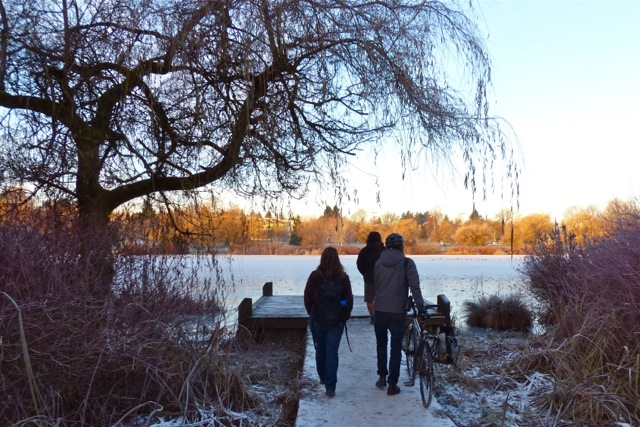
\includegraphics[width=\textwidth]{photos/snowydock}}
\end{figure}
\begin{figure}[h!]
  \centering
  \fbox{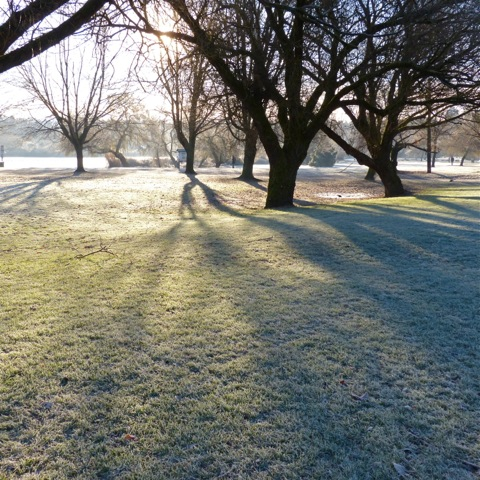
\includegraphics[width=\textwidth]{photos/frosty1}}
\end{figure}
\begin{figure}[b]
  \centering
  \fbox{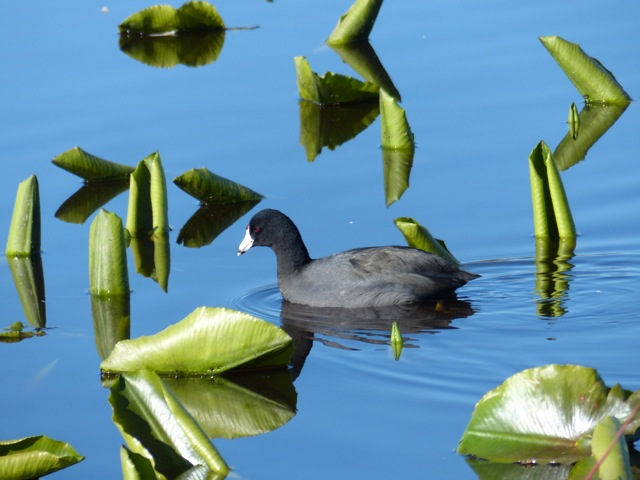
\includegraphics[width=\textwidth]{photos/AMCO}}
  \hspace*{15pt}\hbox{\scriptsize Credit: Philina English}
\end{figure}

